% Circumscribed Parallelepiped
% Author: Axel Pavillet
\documentclass{article}
%%%<
\usepackage{verbatim}
\usepackage{tikz}
\usepackage{tikz-feynman}
\usepackage{adjustbox} % 对齐tikz图用
\usepackage{amsmath,amssymb,amsfonts} % 数学字体
%%%>
\begin{comment}
:Title: Circumscribed Parallelepiped
:Tags: 3D;Geometry;Mathematics
:Author: Axel Pavillet
:Slug: parallelepiped

This is a drawing of a tetrahedron inscibed in a parallelepiped. 
See the following reference p. 58-63 \S 189 to 202

  @BOOK{altshiller1935modern,
    title     = {Modern pure solid geometry},
    publisher = {The Macmillan company},
    year      = {1935},
    author    = {Altshiller-Court, N.},
    address   = {New York},
    edition   = {first},
    lccn      = {35024297},
    url       = {http://books.google.ca/books?id=DDYGAQAAIAAJ}
  }
\end{comment}

\begin{document}

\begin{equation}
  \begin{aligned}
  -i M^2 (p^2)=\text{一圈图}+
  \adjustbox{valign=M}{
    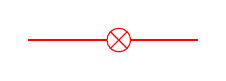
\begin{tikzpicture}[baseline=(current bounding box.base)]
    \begin{feynman} 
    \vertex (a1); 
    \vertex[right=1cm of a1,crossed dot,red] (a2){};
    \vertex[right=1cm of a2] (a3);
    \diagram* { 
    (a1) -- [red] (a2) -- [red] (a3), 
    }; 
    \end{feynman}
    \end{tikzpicture}}
  \end{aligned}
  \end{equation}

\end{document}
